\chapter{Une méthode de composition dynamique de services Web
  sémantiques utilisant Neo4j}
\label{ch:approche}

\section*{Introduction}
\addcontentsline{toc}{section}{Introduction} \markboth{INTRODUCTION}{}

\newpage
\section{Définitions préliminaires}
\label{sec:basic-defs}
Cette section à comme but d'introduire les notions de base ainsi que
les notations et terminologies \ref{sec:basic:ws} employées dans la
suite de ce chapitre, Ensuite nous présentons une formulation
mathématique de notre problème principale, à savoir, \textit{la
  composition des servies Web} sous forme d'un problème de recherche
du plus court chemin dans un graphe orienté
\ref{sec:basic:composition}.\medskip

  \subsection{Services Web}
  \label{sec:basic:ws}
  Chaque web service peut contenir les définitions de différentes
  opérations, identifiables par leur nom, leurs paramètres, Pour des
  raisons de simplicité, nous supposons que chaque service Web
  représente une seule opération.

  \begin{mydef}[\textbf{Service Web}]
    Un Service Web $S$ est un tuple $S = <I,O>$. $I/O$ désigne la
    liste des paramètres ``entrées/sorties'' où chaque paramètre est
    lié à un concept dans l'ontologie du domaine.
   \end{mydef}

  %!TEX root = ../main.tex
\begin{figure}[h]
    \centering
    \includegraphics[width=0.7\textwidth]{figs/ch4/web-service.eps}
    \caption{Un service Web atomique.}
    \label{fig:ch4/web-service}
\end{figure}
%%% Local Variables:
%%% mode: latex
%%% TeX-master: "../../main"
%%% End:


  Nous pouvons donc définir un service comme une application $S$
  définie par:

   \[ S =
     \begin{cases}
       Inputs^n  \to Outputs^m \\
       (i_0, ..., i_n ) \mapsto (o_0, ..., o_m)\\
     \end{cases}
   \]\medskip

   $S$ possède $n$ paramètres d'entrée notés $i_0...i_n$ et $m$
   paramètres de sortie notés $o_0,...o_m$. Dans notre approche
   proposée, nous supposons que chaque service est décrit par un
   document \textit{OWL-S} où chaque paramètre (d'entrée ou de sortie)
   est lié à un concept dans une ontologie \textit{(OWL)} du domaine
   locale.\medskip


   Les ontologies de domaines locales sont les éléments essentiels des
   services web sémantique, créés par les prestataires de services. Un
   fournisseur a besoin de cette classe lorsqu'il crée un service web
   sémantique ainsi que leur ontologie de description (\textit{OWL-S})
   pour pointer les paramètres de ce service vers des entités de cette
   classe.

   \begin{mydef}[\textbf{Annuaire des services Web}]
     un annuaire des services $R$ (ou référentiel des services) est un
     ensemble $R =\{s_0, s_1, ...s_n\}$ des services Web disponibles
     qui peuvent être composés suite à une requête cliente de
     composition.
  \end{mydef}

  Dans notre l'architecture proposé, l'annuaire des services consiste
  à un service Web remplaçant un serveur \acrshort{uddi}. Ce service
  fourni l'ensemble des descriptions \textit{OWL-S} des services
  disponibles, chaque document référence un document \acrshort{wsdl}
  qui à son tour pointe vers l'\acrshort{url} de service décrit
  (\textit{Endpoint}), les descriptions sémantiques des services Web
  disponibles seront stockées dans une base de données relationnelle
  et exposées via un simple interface \acrshort{rest}.\medskip

  %!TEX root = ../../main.tex
\begin{figure}[h]
    \centering
    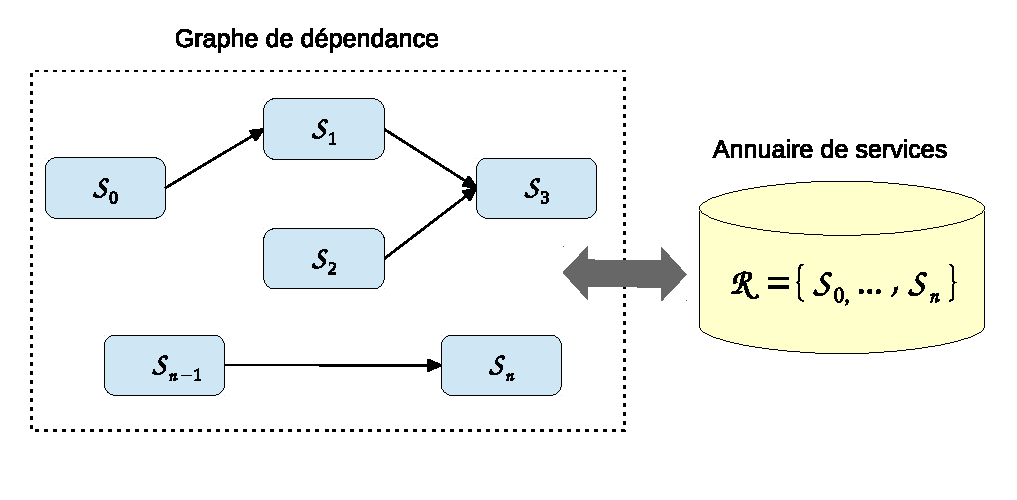
\includegraphics[width=1\textwidth]{figs/ch3/gd.eps}
    \caption{Graphe de dépendance $\mathpzc{GD}$ entre les services
      Web d'un annuaire $\mathpzc{R}$.}
    \label{fig:ch4/gd}
\end{figure}
%%% Local Variables:
%%% mode: latex
%%% TeX-master: "../../main"
%%% End:


  \subsection{Composition de services Web}
  \label{sec:basic:composition}
  Afin de découvrir et sélectionner un service Web composite suite à
  une requête cliente de composition, les services référencés dans un
  annuaire doivent être structurés dans un graphe orienté modélisant
  toutes les relations de dépendance fonctionnelle possibles réalisant
  un \textit{Matching} horizontal \ref{sec:ch4/matching} (la figure
  \ref{fig:ch4/gd}) entre les services disponibles deux par
  deux.\medskip

  \begin{mydef}[\textbf{Graphe de dépendance}]
    Un graphe de dépendance $GD$ est un ``graphe orienté et
    acyclique'' $GD=<R, E_r>$ qui modélise toutes les relations de
    dépendance fonctionnelle possibles entre les services Web
    disponibles dans un annuaire $R$. Il existe une relation $e=(s_0,
    s_1) \in E_r$ si et seulement si il existe une relation de
    dépendance entre $s_0$ et $s_1$.
  \end{mydef}

  L'approche proposée consiste à construire le graphe de dépendance à
  priori (\textit{Offline}) et le sauvegarder dans une base de donnés
  graphe (\textit{Neo4j}). Suite à une requête $Q$, un sous-graphe $G$
  est extrait reflétant un plan de composition exécutable $P$ d'un
  service Web composite satisfaisant.

  \begin{mydef}[\textbf{Requête}]
    Une requête $Q$ est un tuple $Q = <I', O'>$. $I'$ désigne la liste
    des paramètres d'entrée fournis par le client et $O'$ représente
    la listes paramètres requis (sorties).
  \end{mydef}

  %!TEX root = ../../main.tex
\begin{figure}[h]
    \centering
    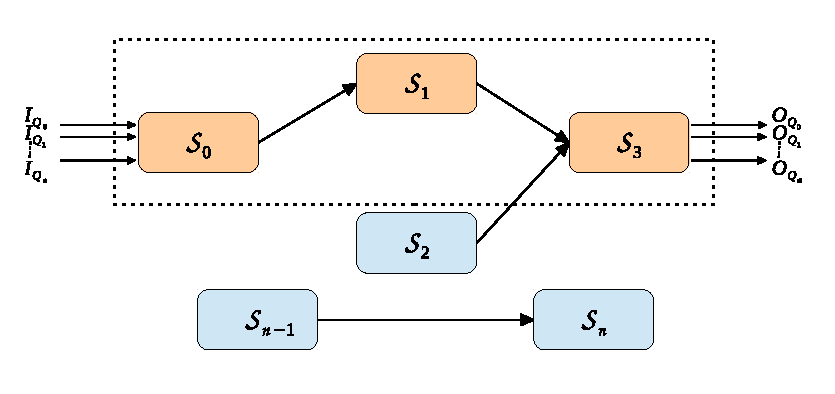
\includegraphics[width=1\textwidth]{figs/ch3/composition-plan.eps}
    \caption{Un service Web composite avec le plan de composition correspond.}
    \label{fig:ch3/composition-plan}
\end{figure}
%%% Local Variables:
%%% mode: latex
%%% TeX-master: "../../main"
%%% End:


  \begin{mydef}[\textbf{Plan de composition}]
    Un plan de composition $P$ est un sous-graphe
    $G$``\textbf{connexe''} d'un graphe de dépendance $GD$, $G=(V,E)$
    tel que $G \subset GD$ décrivant le flux de données/contrôles
    d'exécution d'un ensemble de services Web atomiques $V \subset R$
    engagés dans un processus de composition. Il existe une arête $e
    \in E$ tel que $e = (s_i, s_j)$ si l'exécution d'un service $s_j$
    dépend d'une ou plusieurs paramètres de sorties de $s_i$.
  \end{mydef}

  \begin{mydef}\label{def:ch4/sc}[\textbf{Service Web composite}] Un
    service Web composite $S_c$ est un service Web exécutable composé
    de ``$n$'' services atomique $s \in \{s_0,..., s_n\}$ tel que $n
    \succeq 1$, l'exécution d'un service Web composite correspond à
    l'exécution d'un plan de composition $P$ décrit par $G=<V,E>$ où
    $V = \{s_0, ..., s_n\}$ et $E$ décrivant les relations de
    dépendance entre les services $V$.
  \end{mydef}

  La figure \ref{fig:ch4/composition-plan} représente un service Web
  composite $S_c = <\{i_0, i_1\}, \{o_0, o_1\}>$ correspondant a un
  plan de composition $P$ représenté par un graphe\\ $G =<\{s_0, s_1,
  s_2, s_4\}, \{(s_0, s_1), (s_1, s_2), (s_2, s_4)\}>$.

\section{Matching des services  atomiques}
\label{sec:ch4/matching}

\section{Architecture proposée}
\label{sec:proposition}

\section{Construction et persistance du graphe de dépendance dans une
  base de donnée NeoJ}
\section{Découverte et exécution de services composites}

\section*{Conclusion}
\label{sec:conclusion}
\addcontentsline{toc}{section}{Conclusion} \markboth{CONCLUSION}{}


%%% Local Variables:
%%% mode: latex
%%% TeX-master: "../main"
%%% End:
